\documentclass[12pt]{article}
\usepackage{amsmath}
\usepackage{graphicx}
\usepackage{hyperref}
\usepackage{listings}
\usepackage{color}
\usepackage{pythonhighlight}

\title{Operating System Course Report - First Half of the Semester}
\author{B class}
\date{\today}

\begin{document}

\maketitle
\newpage

\tableofcontents
\newpage

\section{Introduction}
This report summarizes the topics covered during the first half of the Operating System course. It includes theoretical concepts, practical implementations, and assignments. The course focuses on the fundamentals of operating systems, including system architecture, process management, CPU scheduling, and deadlock handling.

\section{Course Overview}
\subsection{Objectives}
The main objectives of this course are:
\begin{itemize}
    \item To understand the basic components and architecture of a computer system.
    \item To learn process management, scheduling, and inter-process communication.
    \item To explore file systems, input/output management, and virtualization.
    \item To study the prevention and handling of deadlocks in operating systems.
\end{itemize}

\subsection{Course Structure}
The course is divided into two halves. This report focuses on the first half, which covers:
\begin{itemize}
    \item Basic Concepts and Components of Computer Systems
    \item System Performance and Metrics
    \item System Architecture of Computer Systems
    \item Process Description and Control
    \item Scheduling Algorithms
    \item Process Creation and Termination
    \item Introduction to Threads
    \item File Systems
    \item Input and Output Management
    \item Deadlock Introduction and Prevention
    \item User Interface Management
    \item Virtualization in Operating Systems
\end{itemize}

\section{Topics Covered}

\subsection{Basic Concepts and Components of Computer Systems}
This section explains the fundamental components that make up a computer system, including the CPU, memory, storage, and input/output devices.

\subsection{System Performance and Metrics}
This section introduces various system performance metrics used to measure the efficiency of a computer system, including throughput, response time, and utilization.

\subsection{System Architecture of Computer Systems}
Describes the architecture of modern computer systems, focusing on the interaction between hardware and the operating system.

\subsection{Process Description and Control}
Processes are a central concept in operating systems. This section covers:
\begin{itemize}
    \item Process states and state transitions
    \item Process control block (PCB)
    \item Context switching
\end{itemize}

\subsection{Scheduling Algorithms}
This section covers:
\begin{itemize}
    \item First-Come, First-Served (FCFS)
    \item Shortest Job Next (SJN)
    \item Round Robin (RR)
\end{itemize}
It explains how these algorithms are used to allocate CPU time to processes.

\subsection{Process Creation and Termination}
Details how processes are created and terminated by the operating system, including:
\begin{itemize}
    \item Process spawning
    \item Process termination conditions
\end{itemize}

\subsection{Introduction to Threads}
This section introduces the concept of threads and their relation to processes, covering:
\begin{itemize}
    \item Single-threaded vs. multi-threaded processes
    \item Benefits of multithreading
\end{itemize}

\begin{figure}[h]
    \centering
    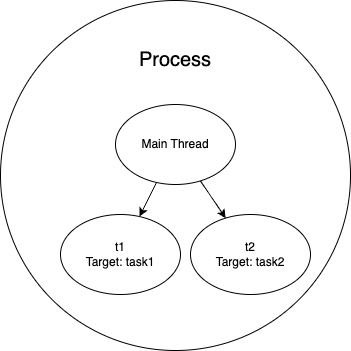
\includegraphics[width=0.5\textwidth]{/Users/khawaritzmi/Unhas/os_report_mid2024/b_class/asset/example.png}  % Sesuaikan nama file dan ukurannya
    \caption{Ini adalah gambar contoh dari multithreading.}
    \label{fig:contoh_gambar}
\end{figure}

Seperti yang terlihat pada Gambar \ref{fig:contoh_gambar}, inilah cara menambahkan gambar dengan keterangan.

\subsection{File Systems}
File systems provide a way for the operating system to store, retrieve, and manage data. This section explains:
\begin{itemize}
    \item File system structure
    \item File access methods
    \item Directory management
\end{itemize}

\subsection{Input and Output Management}
Input and output management is key for handling the interaction between the system and external devices. This section includes:
\begin{itemize}
    \item Device drivers
    \item I/O scheduling
\end{itemize}

\subsection{Deadlock Introduction and Prevention}
Explores the concept of deadlocks and methods for preventing them:
\begin{itemize}
    \item Deadlock prevention techniques
\end{itemize}

\begin{document}

\section*{Definisi Deadlock}
Deadlock merupakan suatu kondisi di mana terdapat dua atau lebih proses yang menunggu untuk mendapatkan resource yang mereka butuhkan tanpa melepaskan resource yang mereka miliki, sehingga terjadi kebuntuan proses.

\section*{Definisi Deadlock Prevention}
Deadlock prevention adalah suatu teknik dalam sistem operasi yang digunakan untuk menghindari terjadinya deadlock dengan memastikan bahwa setidaknya satu dari empat kondisi yang menyebabkan deadlock tidak pernah terpenuhi. Keempat kondisi tersebut meliputi eksklusi mutual (mutual exclusion), tahan dan tunggu (hold and wait), tidak ada pencegahan (no preemption), dan tunggu melingkar (circular wait). Teknik ini biasanya dilakukan dengan mengatur sumber daya dan permintaan proses secara ketat, misalnya dengan menghindari alokasi sumber daya secara eksklusif, atau memastikan bahwa proses tidak menahan sumber daya sambil menunggu sumber daya lain.

\section*{Tujuan}
Tujuan utama dari deadlock prevention adalah untuk mencegah terjadinya deadlock dengan mengeliminasi salah satu dari empat syarat deadlock sebelum terjadinya kondisi tersebut. Ini dilakukan untuk memastikan sistem tetap berjalan tanpa proses yang terganggu oleh sumber daya yang tidak tersedia.

\section*{Kondisi}
\begin{itemize}
    \item \textbf{Mutual Exclusion:} Keadaan di mana setiap sumber daya hanya bisa digunakan untuk satu proses saja pada satu periode tertentu.
    \item \textbf{Hold and Wait:} Suatu keadaan di mana proses dapat masuk ke dalam status hold dan menunggu resource lain yang sedang digunakan proses lain.
    \item \textbf{Non-preemptable:} Suatu sumber daya tidak bisa diambil setiap saat dari suatu proses. Sumber daya hanya dapat diambil apabila proses tersebut telah selesai digunakan.
    \item \textbf{Circular Wait:} Keadaan dua proses saling menunggu secara circular karena proses saling menunggu sumber daya.
\end{itemize}

\section*{Pentingnya Pencegahan Deadlock}
\begin{itemize}
    \item Pencegahan deadlock penting karena dapat meningkatkan efisiensi sistem, memastikan sistem tetap berfungsi optimal tanpa gangguan.
    \item Deadlock mencegah penggunaan sumber daya oleh proses lain, sehingga pencegahannya menghindari pemborosan sumber daya.
    \item Dengan mencegah deadlock, sistem tetap stabil dan tangguh dalam menangani permintaan sumber daya meskipun beban kerja tinggi.
    \item Pencegahan deadlock juga menghindari kegagalan total sistem yang dapat menyebabkan downtime signifikan.
\end{itemize}

\subsection{User Interface Management}
This section discusses the role of the operating system in managing the user interface. Topics covered include:
\begin{itemize}
    \item Graphical User Interface (GUI)
    \item Command-Line Interface (CLI)
    \item Interaction between the user and the operating system
\end{itemize}

\subsection{Virtualization in Operating Systems}
Virtualization allows multiple operating systems to run concurrently on a single physical machine. This section explores:
\begin{itemize}
    \item Concept of virtualization
    \item Hypervisors and their types
    \item Benefits of virtualization in modern computing
\end{itemize}

\section{Assignments and Practical Work}
\subsection{Assignment 1: Process Scheduling}
Students were tasked with implementing various process scheduling algorithms (e.g., FCFS, SJN, and RR) and comparing their performance under different conditions.
\subsubsection{Group 1}
\begin{python}
    class Process:
    def __init__(self, pid, arrival_time, burst_time):
        self.pid = pid
        self.arrival_time = arrival_time
        self.burst_time = burst_time
        self.completion_time = 0
        self.turnaround_time = 0
        self.waiting_time = 0
\end{python}

\begin{table}[htbp]
    \centering
    \begin{tabular}{|c|c|c|} % Defines number of columns and alignment (c = center, l = left, r = right). '|' creates vertical lines.
    \hline
    Header 1 & Header 2 & Header 3 \\ % Column headers
    \hline
    Row 1, Column 1 & Row 1, Column 2 & Row 1, Column 3 \\ % First row of data
    \hline
    Row 2, Column 1 & Row 2, Column 2 & Row 2, Column 3 \\ % Second row of data
    \hline
    \end{tabular}
    \caption{Your table caption} % Optional: For adding a caption
    \label{tab:your_label} % Optional: For cross-referencing the table
\end{table}

\subsection{Assignment 2: Deadlock Handling}
In this assignment, students were asked to simulate different deadlock scenarios and explore various prevention methods.

\subsection{Assignment 3: Multithreading and Amdahl's Law}
This assignment involved designing a multithreading scenario to solve a computationally intensive problem. Students then applied **Amdahl's Law** to calculate the theoretical speedup of the program as the number of threads increased.

\subsection{Assignment 4: Simple Command-Line Interface (CLI) for User Interface Management}
Students were tasked with creating a simple **CLI** for user interface management. The CLI should support basic commands such as file manipulation (creating, listing, and deleting files), process management, and system status reporting.

\subsubsection{Group 10}

\begin{enumerate}

\item Soal

Buatlah sebuah Command-Line Interface (CLI) sederhana yang mendukung perintah untuk pengecekan ketersediaan sumber daya, pengalokasian, dan pelepasan sumber daya, serta strategi pencegahan deadlock.

Berikut adalah contoh implementasi CLI sederhana untuk pencegahan deadlock menggunakan Python.

\textit{JAWABAN: }
\begin{python}
class PengelolaSumberDaya:
    def __init__(self, sumber_daya_t tersedia):
        self.sumber_daya_t tersedia = sumber_daya_t tersedia
        self.sumber_daya_t dialokasikan = {}
        print(f"Sumber daya tersedia awal: {self.sumber_daya_t tersedia}")

    def alokasikan_sumber_daya(self, nama_proses, sumber_daya_diminta):
        if all(self.sumber_daya_t tersedia[i] >= sumber_daya_diminta[i] for i in range(len(sumber_daya_diminta))):
            self.sumber_daya_t tersedia = [self.sumber_daya_t tersedia[i] - sumber_daya_diminta[i] for i in range(len(sumber_daya_diminta))]
            self.sumber_daya_t dialokasikan[nama_proses] = sumber_daya_diminta
            print(f"Sumber daya dialokasikan ke {nama_proses}: {sumber_daya_diminta}")
            print(f"Sumber daya tersedia yang tersisa: {self.sumber_daya_t tersedia}")
        else:
            print(f"Tidak dapat mengalokasikan sumber daya ke {nama_proses}. Sumber daya tidak cukup tersedia.")

    def lepas_sumber_daya(self, nama_proses):
        if nama_proses in self.sumber_daya_t dialokasikan:
            sumber_daya_yang_dilepas = self.sumber_daya_t dialokasikan.pop(nama_proses)
            self.sumber_daya_t tersedia = [self.sumber_daya_t tersedia[i] + sumber_daya_yang_dilepas[i] for i in range(len(sumber_daya_yang_dilepas))]
            print(f"Sumber daya dilepas oleh {nama_proses}: {sumber_daya_yang_dilepas}")
            print(f"Sumber daya tersedia yang tersisa: {self.sumber_daya_t tersedia}")
        else:
            print(f"Tidak ada sumber daya yang dialokasikan untuk {nama_proses}.")

    def status_sistem(self):
        print(f"Sumber daya tersedia: {self.sumber_daya_t tersedia}")
        print(f"Sumber daya dialokasikan: {self.sumber_daya_t dialokasikan}")

def antarmuka_cli():
    sumber_daya_t tersedia = [10, 5, 7]  # Contoh: 10 sumber daya A, 5 sumber daya B, 7 sumber daya C
    pg = PengelolaSumberDaya(sumber_daya_t tersedia)

    while True:
        print("\n--- Menu CLI Pencegahan Deadlock ---")
        print("1. Alokasikan Sumber Daya")
        print("2. Lepas Sumber Daya")
        print("3. Cek Status Sistem")
        print("4. Keluar")

        pilihan = input("Masukkan pilihan Anda: ")

        if pilihan == "1":
            nama_proses = input("Masukkan nama proses: ")
            sumber_daya_diminta = list(map(int, input("Masukkan sumber daya yang diminta (misal, 2 1 3): ").split()))
            pg.alokasikan_sumber_daya(nama_proses, sumber_daya_diminta)
        elif pilihan == "2":
            nama_proses = input("Masukkan nama proses untuk melepas sumber daya: ")
            pg.lepas_sumber_daya(nama_proses)
        elif pilihan == "3":
            pg.status_sistem()
        elif pilihan == "4":
            print("Keluar dari CLI.")
            break
        else:
            print("Pilihan tidak valid. Silakan coba lagi.")

if __name__ == "__main__":
    antarmuka_cli()
\end{python}

\textit{PENJELASAN: }
\begin{enumerate}
    \item Fungsi CLI untuk pencegahan deadlock meliputi:
        \begin{enumerate}
            \item \textbf{allocate\_resources}: Memeriksa ketersediaan sumber daya sebelum mengalokasikan ke proses tertentu. Jika sumber daya yang diminta tersedia, sumber daya dialokasikan, dan ini membantu mencegah deadlock dengan strategi pencegahan deadlock berbasis alokasi sumber daya.
            \item \textbf{release\_resources}: Melepaskan sumber daya dari proses tertentu dan mengembalikannya ke sistem. Hal ini juga membantu dalam strategi pencegahan deadlock dengan pelepasan sumber daya tepat waktu.
            \item \textbf{system\_status}: Menampilkan status sumber daya saat ini (tersedia dan dialokasikan). Ini memberikan gambaran tentang bagaimana sumber daya dikelola dalam sistem, yang penting untuk mencegah deadlock.
        \end{enumerate}
    \item Fungsi utama, \textbf{cli\_interface}, menampilkan menu dan memungkinkan pengguna untuk mengelola sumber daya, termasuk mengalokasikan dan melepaskan sumber daya. Ini menunjukkan cara sistem dapat menghindari deadlock melalui manajemen yang tepat.
    \item Pengguna dapat:
        \begin{enumerate}
            \item Mengalokasikan sumber daya ke proses.
            \item Melepaskan sumber daya dari proses.
            \item Mengecek status sumber daya sistem.
            \item Keluar dari program.
        \end{enumerate}
    \item CLI ini menggunakan konsep pencegahan deadlock dengan memastikan bahwa permintaan sumber daya hanya diberikan jika sumber daya yang diminta tersedia, dan memastikan sumber daya dilepas secara tepat.
\end{enumerate}
\end{enumerate}

\subsection{Assignment 5: File System Access}
In this assignment, students implemented file system access routines, including:
\begin{itemize}
    \item File creation and deletion
    \item Reading from and writing to files
    \item Navigating directories and managing file permissions
\end{itemize}

\section{Conclusion}
The first half of the course introduced core operating system concepts, including process management, scheduling, multithreading, and file system access. These topics provided a foundation for more advanced topics to be covered in the second half of the course.

\begin{thebibliography}{3}

    \bibitem{}
    Safei, T. T. Pencegahan Deadlock pada Alokasi Resource dalam Sistem Operasi Menggunakan Algoritma Greedy.
    
    \bibitem{}
    Viswanadham, N., Narahari, Y., and Johnson, T. L. (1990). Deadlock prevention and deadlock avoidance in flexible manufacturing systems using Petri net models. IEEE Transactions on Robotics and Automation Magazine, 6(6), 713-723.
    
    \bibitem{}
    Mumtahana, S. H. A. (2018). Implementasi Penanganan Deadlock Menggunakan Metode Taskkill. TRANSFORMASI, 13(2).
    
    \bibitem{}
    Prasetiyo, S. M., Gustiawan, R., and Albani, F. R. (2024). Penanganan Deadlock Yang Optimal Dalam Sistem Operasi Windows: Pencegahan, Identifikasi Penyebab, Dan Konsekuensi Deadlock. Buletin Ilmiah Ilmu Komputer dan Multimedia (BIIKMA), 2(1), 60-64.
    \end{thebibliography}
\end{document}